\documentclass[12pt,letterpaper]{article}

% --- 1. CONFIGURACIÓN DE IDIOMA Y CARACTERES ---
\usepackage[utf8]{inputenc}
\usepackage[T1]{fontenc}
\usepackage[spanish, es-nodecimaldot, es-noquoting]{babel}
\usepackage{csquotes}
\usepackage{mathpazo}          % Palatino para texto y matemáticas
\usepackage{textcomp}
\usepackage{microtype}

% --- 2. GEOMETRÍA ---
\usepackage[margin=2.5cm, headheight=14pt]{geometry}

% --- 3. ESPACIADO ENTRE PÁRRAFOS ---
\setlength{\parskip}{0.6em}
\setlength{\parindent}{0pt}

% --- 4. MATEMÁTICAS ---
\usepackage{amsmath,amssymb}

% --- 5. TABLAS Y GRÁFICOS ---
\usepackage{booktabs}
\usepackage{array}
\usepackage{colortbl}
\usepackage{xcolor}
\usepackage{graphicx}
\usepackage{float}
\usepackage{pifont}
\usepackage{multirow}

% --- 6. CAJAS Y ENTORNOS ---
\usepackage{tcolorbox}
\tcbuselibrary{skins,breakable}

% --- 7. ENCABEZADOS Y PIES ---
\usepackage{fancyhdr}
\pagestyle{fancy}
\fancyhf{}
\fancyhead[L]{\small\textsc{Optimización Inteligente --- Fase 3}}
\fancyhead[R]{\small\textsc{MIAAD \textcolor{uacjgray}{\textbullet} UACJ}}
\fancyfoot[C]{\thepage}
\renewcommand{\headrulewidth}{0.4pt}

% --- 8. HIPERVÍNCULOS ---
\usepackage{hyperref}
\hypersetup{colorlinks=true, linkcolor=blue!60!black, urlcolor=blue!60!black, citecolor=blue!60!black}

% --- 9. COLORES PERSONALIZADOS ---
\definecolor{headerblue}{HTML}{003CA6}
\definecolor{uacjyellow}{HTML}{FFD600}
\definecolor{sectiongreen}{HTML}{27AE60}
\definecolor{formulabg}{HTML}{F1F8E9}
\definecolor{formulaborder}{HTML}{DCEDC8}
\definecolor{restrictionbg}{HTML}{FFF3E0}
\definecolor{restrictionborder}{HTML}{FF9800}
\definecolor{deliverbg}{HTML}{E3F2FD}
\definecolor{tablehead}{HTML}{2C3E50}
\definecolor{uacjgray}{HTML}{555559}
\definecolor{alertred}{HTML}{B41E1E}
\definecolor{answerbg}{HTML}{E8F5E9}
\definecolor{answerborder}{HTML}{2E7D32}
\definecolor{examplebg}{HTML}{FFF8E1}
\definecolor{exampleborder}{HTML}{F9A825}

% --- 10. CAJAS TCOLORBOX ---
\newtcolorbox{formulabox}{
    colback=formulabg,
    colframe=formulaborder,
    arc=4pt,
    boxrule=0.8pt,
    left=8pt, right=8pt, top=8pt, bottom=8pt
}

\newtcolorbox{restrictionbox}{
    colback=restrictionbg,
    colframe=restrictionborder,
    borderline west={3pt}{0pt}{restrictionborder},
    arc=2pt,
    boxrule=0.5pt,
    left=10pt, right=10pt, top=8pt, bottom=8pt
}

\newtcolorbox{notebox}[1][]{
    colback=deliverbg,
    colframe=headerblue!40,
    borderline west={4pt}{0pt}{headerblue},
    arc=2pt,
    boxrule=0.5pt,
    left=10pt, right=10pt, top=8pt, bottom=8pt,
    #1
}

\newtcolorbox{resultbox}[1][]{
    colback=formulabg,
    colframe=sectiongreen!60,
    borderline west={4pt}{0pt}{sectiongreen},
    arc=2pt,
    boxrule=0.5pt,
    left=10pt, right=10pt, top=8pt, bottom=8pt,
    #1
}

\newtcolorbox{yellowbox}[1][]{
    colback=uacjyellow!10,
    colframe=uacjyellow!50,
    borderline west={4pt}{0pt}{uacjyellow},
    arc=2pt,
    boxrule=0.5pt,
    left=10pt, right=10pt, top=8pt, bottom=8pt,
    #1
}

\newtcolorbox{answerbox}[1][]{
    colback=answerbg,
    colframe=answerborder,
    borderline west={4pt}{0pt}{answerborder},
    arc=2pt,
    boxrule=0.5pt,
    left=10pt, right=10pt, top=8pt, bottom=8pt,
    #1
}

\newtcolorbox{examplebox}[1][]{
    colback=examplebg,
    colframe=exampleborder,
    borderline west={4pt}{0pt}{exampleborder},
    arc=2pt,
    boxrule=0.5pt,
    left=10pt, right=10pt, top=8pt, bottom=8pt,
    #1
}

% --- 11. SECCIONES CON LÍNEA DORADA ---
\usepackage{titlesec}
\titleformat{\section}
    {\Large\bfseries\color{headerblue}}
    {\thesection.}{0.5em}{}
    [\vspace{-0.5em}{\color{uacjyellow}\rule{5pt}{0pt}\rule[0.3ex]{0.4\linewidth}{2pt}}]

\titleformat{\subsection}
    {\large\bfseries\color{headerblue}}
    {\thesubsection.}{0.5em}{}

\titleformat{\subsubsection}
    {\normalsize\bfseries\color{headerblue!80}}
    {\thesubsubsection.}{0.5em}{}

% --- 12. RUTA DE FIGURAS ---
\graphicspath{{../results/figures/}{Figures/}}

% --- 13. BIBLIOGRAFÍA APA 7 ---
\usepackage[style=apa, backend=biber, language=spanish, sortcites=true, sorting=nyt]{biblatex}
\DeclareLanguageMapping{spanish}{spanish-apa}

\begin{filecontents}[overwrite]{referencias_fase3.bib}
@article{bean1994,
  author    = {Bean, James C.},
  title     = {Genetic algorithms and random keys for sequencing and optimization},
  journal   = {ORSA Journal on Computing},
  year      = {1994},
  volume    = {6},
  number    = {2},
  pages     = {154--160},
  doi       = {10.1287/ijoc.6.2.154}
}
@article{heidari2019,
  author    = {Heidari, Ali Asghar and Mirjalili, Seyedali and Faris, Hossam and Aljarah, Ibrahim and Mafarja, Majdi and Chen, Huiling},
  title     = {Harris hawks optimization: Algorithm and applications},
  journal   = {Future Generation Computer Systems},
  year      = {2019},
  volume    = {97},
  pages     = {849--872},
  doi       = {10.1016/j.future.2019.02.028}
}
@article{kusoglu2020,
  author    = {Ku{\c{s}}o{\u{g}}lu, {\.{I}}lyas and Y{\"u}zge{\c{c}}, Ufuk},
  title     = {Multi-objective {Harris Hawks} optimizer for multiobjective optimization problems},
  journal   = {BSEU Journal of Engineering Research and Technology},
  year      = {2020},
  volume    = {1},
  number    = {1},
  pages     = {1--12}
}
@article{cerci2022,
  author    = {{\c{C}}er{\c{c}}i, Sezer and D{\"o}nmez, Erkan},
  title     = {Hybrid multi-objective {Harris Hawk} optimization algorithm based on elite non-dominated sorting and grid index mechanism},
  journal   = {Advances in Engineering Software},
  year      = {2022},
  volume    = {173},
  pages     = {103214},
  doi       = {10.1016/j.advengsoft.2022.103214}
}
@misc{crs2023,
  author    = {{Congressional Research Service}},
  title     = {{U.S.} employment-based immigration policy},
  year      = {2023},
  note      = {R47164},
  url       = {https://www.congress.gov/crs-product/R47164}
}
@misc{dosfeb2026,
  author    = {{U.S. Department of State}},
  title     = {Visa bulletin for {February} 2026},
  year      = {2026},
  url       = {https://travel.state.gov/content/travel/en/legal/visa-law0/visa-bulletin/2026/visa-bulletin-for-february-2026.html}
}
@misc{uscis2023,
  author    = {{U.S. Citizenship and Immigration Services}},
  title     = {Fiscal year 2023 employment-based adjustment of status {FAQs}},
  year      = {2023},
  url       = {https://www.uscis.gov/green-card/green-card-processes-and-procedures/fiscal-year-2023-employment-based-adjustment-of-status-faqs}
}
@misc{fwd2024,
  author    = {{FWD.us}},
  title     = {Per-country cap reform: Priority bill spotlight},
  year      = {2024},
  url       = {https://www.fwd.us/news/per-country-cap-reform-priority-bill-spotlight/}
}
@book{gareyjohnson1979,
  author    = {Garey, Michael R. and Johnson, David S.},
  title     = {Computers and Intractability: A Guide to the Theory of {NP}-Completeness},
  year      = {1979},
  publisher = {W. H. Freeman},
  address   = {San Francisco}
}
\end{filecontents}
\addbibresource{referencias_fase3.bib}

% ==========================================================
\begin{document}

% ==========================================
% PORTADA
% ==========================================
\begin{titlepage}
\begin{center}

    \vspace*{0.5cm}

    
\includegraphics[width=2.5cm]{logo_miaad.png}

    \vspace{0.5cm}

    {\large\bfseries\scshape Universidad Autónoma de Ciudad Juárez}\\[4pt]
    {\normalsize Instituto de Ingeniería y Tecnología}\\[2pt]
    {\normalsize Departamento de Ingeniería Eléctrica y Computación}

    \vspace{0.6cm}

    {\Large\bfseries\scshape\color{headerblue} Maestría en Inteligencia Artificial\\[4pt] y Analítica de Datos}

    \vspace{0.4cm}

    {\color{uacjgray}\hrule height 0.8pt}
    \vspace{0.2cm}
    {\color{uacjyellow}\hrule height 2.5pt}

    \vfill

    {\large\textsc{Optimización Inteligente}}\\[4pt]
    {\small Mtro.~Raúl Gibrán Porras Alaniz}

    \vspace{0.5cm}

    \begin{tcolorbox}[
        colback=headerblue!6,
        colframe=headerblue,
        boxrule=1.2pt,
        arc=5pt,
        width=0.9\textwidth,
        halign=center,
        top=4mm,
        bottom=4mm
    ]
        {\Large\bfseries\color{headerblue} Proyecto Final: Fase 03}\\[6pt]
        {\large\bfseries Implementación y Resultados}\\[8pt]
        {\normalsize\bfseries Optimización Multiobjetivo de la Asignación de}\\[3pt]
        {\normalsize\bfseries \textit{Green Cards} en Estados Unidos mediante}\\[3pt]
        {\normalsize\bfseries Harris Hawks Optimization (HHO)}\\[6pt]
        {\small\color{uacjgray} Nombre del proyecto: \textbf{Visa Predict AI}}
    \end{tcolorbox}

    \vfill

    {\normalsize\textbf{Equipo:}}\\[6pt]
    {\normalsize Yazmín Ivonne Flores Martínez \textcolor{uacjgray}{\textbullet} \textit{261548}}\\[3pt]
    {\normalsize Javier Augusto Rebull Saucedo \textcolor{uacjgray}{\textbullet} \textit{263483}}

    \vspace{0.8cm}

    {\normalsize\textbf{Fecha de Entrega:}}\\[4pt]
    {\normalsize Marzo de 2026}

    \vspace{1.0cm}

\end{center}
\end{titlepage}

% ==========================================
% TABLA DE CONTENIDOS
% ==========================================
\tableofcontents
\newpage

% ==========================================================
% SECCION 1. RESUMEN DE CORRECCIONES AL MODELO
% ==========================================================
\section{Resumen de Correcciones al Modelo}
\label{sec:correcciones}

Previo a la implementación, se identificaron seis brechas (gaps) entre la formulación de la Fase~02 y los requisitos de rigor necesarios para una implementación reproducible. Esta sección documenta cada brecha y la corrección aplicada.

\subsection{G1: Formulación compacta del problema biobjetivo}

\begin{notebox}
\textbf{Brecha detectada:} La Fase~02 presentó los dos objetivos y las restricciones de forma narrativa, pero no incluyó una formulación compacta estándar que permita a cualquier lector identificar de un vistazo la estructura del problema.
\end{notebox}

\textbf{Corrección.} Se enuncia la formulación compacta del problema biobjetivo:

\begin{formulabox}
\begin{align}
\min_{\mathbf{x}} \quad & \bigl\{ f_1(\mathbf{x}),\; f_2(\mathbf{x}) \bigr\} \label{eq:compact}\\[6pt]
\text{s.a.} \quad
& \text{R1: } \sum_{g \in \mathcal{G}} x_g \leq V \notag\\
& \text{R2: } \sum_{g:\,c(g)=c} x_g \leq P_c \quad \forall\, c \in \mathcal{C} \notag\\
& \text{R3: } \sum_{g:\,j(g)=j} x_g \leq K_j^{\text{eff}} \quad \forall\, j \in \mathcal{J} \notag\\
& \text{R4: } 0 \leq x_g \leq n_g \quad \forall\, g \in \mathcal{G} \notag\\
& \text{R5: } x_g \in \mathbb{Z}^{+}_0 \quad \forall\, g \in \mathcal{G} \notag\\
& \text{R6: FIFO por } (c, j) \notag
\end{align}

donde $f_1(\mathbf{x}) = \frac{\sum_{g}(n_g - x_g)\,w_g}{\sum_{g} n_g}$ es la carga de espera no atendida y $f_2(\mathbf{x}) = \max_{c_1,c_2}|\bar{W}_{c_1} - \bar{W}_{c_2}|$ es la máxima disparidad entre países.
\end{formulabox}

Esta formulación hace explícito que se trata de un problema de optimización combinatoria biobjetivo con seis restricciones, perteneciente a la clase NP-Difícil \parencite{gareyjohnson1979}.

\subsection{G2: Prueba formal de conflicto entre $f_1$ y $f_2$}

\begin{notebox}
\textbf{Brecha detectada:} La Fase~02 afirmó que $f_1$ y $f_2$ están en conflicto, pero no proporcionó una demostración formal con soluciones concretas.
\end{notebox}

\textbf{Corrección.} Se construyen dos permutaciones concretas que producen soluciones mutuamente no dominadas:

\begin{examplebox}
\textbf{Permutación $\boldsymbol{\pi}_A$:} Prioriza los grupos con mayor $w_g$ (India-EB2, India-EB3, etc.). Resultado: $f_1(\mathbf{x}_A) = 8{,}05$, $f_2(\mathbf{x}_A) = 12{,}00$ años.

\textbf{Permutación $\boldsymbol{\pi}_B$:} Distribuye visas equitativamente entre todos los países. Resultado: $f_1(\mathbf{x}_B) = 8{,}30$, $f_2(\mathbf{x}_B) = 2{,}88$ años.

\textbf{Conclusión:} $\mathbf{x}_A$ domina a $\mathbf{x}_B$ en $f_1$ ($8{,}05 < 8{,}30$), pero $\mathbf{x}_B$ domina a $\mathbf{x}_A$ en $f_2$ ($2{,}88 < 12{,}00$). Ninguna domina a la otra $\Rightarrow$ son mutuamente no dominadas, confirmando que $f_1$ y $f_2$ están en conflicto. \ding{51}
\end{examplebox}

\subsection{G3: Definición formal del frente de Pareto}

\begin{notebox}
\textbf{Brecha detectada:} No se definió formalmente el concepto de dominancia de Pareto ni el frente de Pareto.
\end{notebox}

\textbf{Corrección.} Se adoptan las definiciones estándar:

\begin{formulabox}
\textbf{Dominancia de Pareto.} Una solución $\mathbf{x}$ domina a $\mathbf{x}'$ (denotado $\mathbf{x} \prec \mathbf{x}'$) si y solo si:
\[
\forall\, i \in \{1,2\}:\; f_i(\mathbf{x}) \leq f_i(\mathbf{x}') \quad \wedge \quad \exists\, i \in \{1,2\}:\; f_i(\mathbf{x}) < f_i(\mathbf{x}')
\]

\textbf{Frente de Pareto.} El conjunto de soluciones no dominadas del espacio factible $\mathcal{F}$:
\[
\mathcal{P}^* = \bigl\{\mathbf{x} \in \mathcal{F} \;\big|\; \nexists\, \mathbf{x}' \in \mathcal{F} : \mathbf{x}' \prec \mathbf{x}\bigr\}
\]
\end{formulabox}

El objetivo de MOHHO es aproximar $\mathcal{P}^*$ mediante un archivo externo de soluciones no dominadas.

\subsection{G4: Parámetro $w_g$ en tabla de parámetros}

\begin{notebox}
\textbf{Brecha detectada:} El peso de espera $w_g = t_{\text{actual}} - d_g$ se usó en las funciones objetivo, pero no aparecía explícitamente en la tabla de parámetros de la Fase~02.
\end{notebox}

\textbf{Corrección.} Se añade $w_g$ a la tabla de parámetros del modelo:

\begin{table}[H]
\centering
\renewcommand{\arraystretch}{1.3}
\begin{tabular}{clp{6cm}l}
\toprule
\rowcolor{tablehead}
\textcolor{white}{\textbf{Símbolo}} & \textcolor{white}{\textbf{Nombre}} & \textcolor{white}{\textbf{Descripción}} & \textcolor{white}{\textbf{Ejemplo}} \\
\midrule
$w_g$ & Peso de espera & $w_g = t_{\text{actual}} - d_g$, tiempo de espera del grupo $g$ en años & $w_g = 2026 - 2013 = 13$ \\
\bottomrule
\end{tabular}
\end{table}

\subsection{G5: Cita formal de SPV (Bean, 1994)}

\begin{notebox}
\textbf{Brecha detectada:} La regla SPV (\textit{Smallest Position Value}) se describió en la Fase~02, pero no se citó la referencia original.
\end{notebox}

\textbf{Corrección.} La regla SPV fue propuesta por \textcite{bean1994} en el contexto de algoritmos genéticos con \textit{random keys}. El principio consiste en representar una permutación mediante un vector de claves reales $\mathbf{H} \in \mathbb{R}^G$ y obtener la permutación $\boldsymbol{\pi}$ ordenando los índices por valor ascendente de $h_g$. Esta representación permite que operadores diseñados para espacios continuos (como los de HHO) generen permutaciones válidas de forma natural, sin necesidad de operadores de reparación.

\subsection{G6: Precisión en la descripción del decodificador}

\begin{notebox}
\textbf{Brecha detectada:} La Fase~02 describió el decodificador como un proceso que <<asigna visas grupo por grupo>>, pero no especificó con precisión las condiciones de parada ni el manejo del residuo.
\end{notebox}

\textbf{Corrección.} El decodificador greedy procesa los grupos en el orden dado por la permutación $\boldsymbol{\pi}$. Para cada grupo $g = \pi_k$, se calcula la asignación máxima factible:
\[
x_g = \min\!\Big(n_g,\; V_{\text{res}},\; P_{c(g)}^{\text{res}},\; K_{j(g)}^{\text{res}}\Big)
\]
donde $V_{\text{res}}$, $P_{c(g)}^{\text{res}}$ y $K_{j(g)}^{\text{res}}$ son los residuos actualizados de las restricciones R1, R2 y R3, respectivamente. Después de cada asignación, se decrementan los tres contadores residuales. El proceso termina cuando $V_{\text{res}} = 0$ o se han procesado los $G$ grupos. Toda solución decodificada satisface R1--R6 por construcción.

% ==========================================================
% SECCION 2. IMPLEMENTACIÓN
% ==========================================================
\newpage
\section{Implementación}
\label{sec:implementacion}

\subsection{Arquitectura general}

La implementación se realizó en \textbf{Python 3.11} con una arquitectura modular que separa claramente el modelo del problema, el algoritmo de optimización y el análisis de resultados. La estructura de directorios sigue el patrón:

\begin{table}[H]
\centering
\caption{Módulos principales de la implementación.}
\label{tab:modulos}
\renewcommand{\arraystretch}{1.4}
\begin{tabular}{lp{8cm}}
\toprule
\rowcolor{tablehead}
\textcolor{white}{\textbf{Módulo}} & \textcolor{white}{\textbf{Responsabilidad}} \\
\midrule
\texttt{problem.py} & Define los datos del problema (países, categorías, demanda, topes), las funciones objetivo $f_1$ y $f_2$, y el decodificador greedy. \\
\rowcolor{gray!8}
\texttt{mohho.py} & Implementa el algoritmo Multi-Objective Harris Hawks Optimization con archivo externo de soluciones no dominadas. \\
\texttt{spv.py} & Implementa la regla SPV \parencite{bean1994}: convierte vectores continuos en permutaciones. \\
\rowcolor{gray!8}
\texttt{archive.py} & Gestión del archivo externo: inserción, dominancia, poda por \textit{crowding distance}. \\
\texttt{experiment.py} & Orquesta las 30 corridas independientes, recolecta métricas y genera el frente combinado. \\
\rowcolor{gray!8}
\texttt{analysis.py} & Calcula estadísticas (hipervolumen, \textit{spacing}, \textit{spread}) y genera las figuras del reporte. \\
\bottomrule
\end{tabular}
\end{table}

\subsection{Diseño del algoritmo MOHHO}

El algoritmo Multi-Objective Harris Hawks Optimization (MOHHO) extiende el HHO original \parencite{heidari2019} al caso multiobjetivo siguiendo la estrategia de \textcite{kusoglu2020}, complementada con las mejoras de archivo de \textcite{cerci2022}. Las adaptaciones principales son:

\begin{enumerate}
    \item \textbf{Selección del líder (presa):} En lugar de un único óptimo global, el líder se selecciona aleatoriamente del archivo externo de soluciones no dominadas, con probabilidad inversamente proporcional a la \textit{crowding distance} para favorecer la diversidad.

    \item \textbf{Archivo externo:} Almacena hasta 100 soluciones no dominadas. Cuando se excede la capacidad, se eliminan las soluciones con menor \textit{crowding distance} (mayor densidad local en el espacio objetivo).

    \item \textbf{Actualización de no dominancia:} Después de cada iteración, las nuevas soluciones se comparan con el archivo. Si una nueva solución no es dominada por ningún miembro del archivo, se inserta y se eliminan las soluciones que ella domine.

    \item \textbf{Decodificación SPV:} Cada halcón $\mathbf{H} \in \mathbb{R}^{50}$ se convierte en permutación mediante SPV \parencite{bean1994}, se decodifica con el greedy, y se evalúan $f_1$ y $f_2$ sobre la asignación resultante.
\end{enumerate}

\subsection{Flujo del algoritmo}

\begin{resultbox}
\textbf{Pseudocódigo simplificado de MOHHO:}

\begin{enumerate}
    \item Inicializar $N = 50$ halcones aleatorios en $\mathbb{R}^{50}$.
    \item Decodificar cada halcón (SPV $\to$ permutación $\to$ greedy $\to$ asignación).
    \item Evaluar $(f_1, f_2)$ y construir el archivo inicial de no dominados.
    \item \textbf{Para} $t = 1$ hasta $T = 500$:
    \begin{enumerate}
        \item Calcular la energía de escape $E_0 \sim U(-1, 1)$ y $E = 2\,E_0\,(1 - t/T)$.
        \item Seleccionar líder del archivo (por \textit{crowding distance}).
        \item \textbf{Para} cada halcón $i$:
        \begin{itemize}
            \item Si $|E| \geq 1$: fase de exploración (salto de Lévy o posición aleatoria).
            \item Si $|E| < 1$: fase de explotación (asedio suave/duro, con o sin inmersión rápida).
        \end{itemize}
        \item Decodificar y evaluar cada halcón actualizado.
        \item Actualizar el archivo de no dominados.
    \end{enumerate}
    \item Retornar el archivo final como aproximación al frente de Pareto.
\end{enumerate}
\end{resultbox}

\subsection{Decisiones de diseño relevantes}

\begin{yellowbox}
\textbf{Factibilidad garantizada.} No se implementan funciones de penalización. El decodificador greedy garantiza que \textbf{toda} solución decodificada satisface las restricciones R1--R6. Los operadores de HHO operan libremente en $\mathbb{R}^{50}$ sin necesidad de reparación; la factibilidad se maneja exclusivamente en la capa de decodificación.
\end{yellowbox}

\begin{yellowbox}
\textbf{Reproducibilidad.} Cada una de las 30 corridas utiliza una semilla aleatoria distinta (semillas 1 a 30). Los datos de entrada, parámetros y código fuente están versionados en el repositorio del proyecto.
\end{yellowbox}

% ==========================================================
% SECCION 3. CONFIGURACIÓN EXPERIMENTAL
% ==========================================================
\newpage
\section{Configuración Experimental}
\label{sec:config}

\subsection{Parámetros del algoritmo}

\begin{table}[H]
\centering
\caption{Parámetros de configuración de MOHHO.}
\label{tab:parametros_mohho}
\renewcommand{\arraystretch}{1.4}
\begin{tabular}{lll}
\toprule
\rowcolor{tablehead}
\textcolor{white}{\textbf{Parámetro}} & \textcolor{white}{\textbf{Valor}} & \textcolor{white}{\textbf{Justificación}} \\
\midrule
Tamaño de población ($N$) & 50 & Igual a la dimensión del problema ($G = 50$) \\
\rowcolor{gray!8}
Iteraciones máximas ($T$) & 500 & Convergencia observada antes de la iteración 300 \\
Tamaño de archivo & 100 & Balance entre diversidad y costo computacional \\
\rowcolor{gray!8}
Corridas independientes & 30 & Estándar en la literatura para significancia estadística \\
Dimensión ($G$) & 50 & $C \times |\mathcal{J}| = 10 \times 5$ grupos \\
\rowcolor{gray!8}
Energía inicial $E_0$ & $U(-1, 1)$ & Distribución estándar de HHO \parencite{heidari2019} \\
Selector de líder & \textit{Crowding distance} & Favorece diversidad en el frente \\
\rowcolor{gray!8}
Poda de archivo & \textit{Crowding distance} & Elimina soluciones en regiones densas \\
\bottomrule
\end{tabular}
\end{table}

\subsection{Datos de entrada del problema}

Los datos del problema corresponden al año fiscal 2026, con la siguiente configuración:

\begin{itemize}
    \item \textbf{Visas totales EB:} $V = 140.000$.
    \item \textbf{Países representativos:} $C = 10$ (India, China, Filipinas, México, Corea del Sur, Brasil, Canadá, Reino Unido, Nigeria, Resto del Mundo).
    \item \textbf{Categorías:} $|\mathcal{J}| = 5$ (EB-1 a EB-5).
    \item \textbf{Grupos:} $G = 50$ combinaciones país-categoría.
    \item \textbf{Tope por país:} $P_c = 25.620$ visas (7\% de 366.000) \parencite{crs2023}.
    \item \textbf{Demanda:} Datos de backlog estimados a partir de los \textit{Visa Bulletins} \parencite{dosfeb2026} y reportes de USCIS \parencite{uscis2023}.
\end{itemize}

\subsection{Métricas de evaluación}

Se utilizan las siguientes métricas para evaluar la calidad de las aproximaciones al frente de Pareto:

\begin{table}[H]
\centering
\caption{Métricas de desempeño.}
\label{tab:metricas}
\renewcommand{\arraystretch}{1.4}
\begin{tabular}{lp{9cm}}
\toprule
\rowcolor{tablehead}
\textcolor{white}{\textbf{Métrica}} & \textcolor{white}{\textbf{Descripción}} \\
\midrule
Hipervolumen (HV) & Volumen del espacio objetivo dominado por el frente aproximado respecto a un punto de referencia. Mayor HV indica mejor convergencia y diversidad. \\
\rowcolor{gray!8}
Número de soluciones no dominadas & Cardinalidad del frente aproximado. Más soluciones ofrecen más opciones al tomador de decisiones. \\
Frente combinado & Unión de los frentes de las 30 corridas, filtrada por no dominancia, para estimar el frente global. \\
\bottomrule
\end{tabular}
\end{table}

\subsection{Baseline: Sistema FIFO actual}

Para comparar con el sistema vigente, se implementó el decodificador greedy con la permutación FIFO pura: los grupos se ordenan por fecha de prioridad $d_g$ ascendente (los más antiguos primero). Esta permutación es determinista y produce una única asignación de referencia:

\begin{resultbox}
\textbf{Resultado FIFO:} $f_1 = 8{,}0854$, \; $f_2 = 13{,}0000$ años.

El sistema actual logra una carga de espera moderada ($f_1 = 8{,}09$) porque prioriza a los grupos más antiguos, pero genera la \textbf{máxima disparidad posible} ($f_2 = 13{,}00$) al concentrar las visas en pocos países sobredemandados e ignorar la equidad entre nacionalidades.
\end{resultbox}

% ==========================================================
% SECCION 4. RESULTADOS
% ==========================================================
\newpage
\section{Resultados}
\label{sec:resultados}

\subsection{Frente de Pareto combinado}

Tras las 30 corridas independientes, se combinaron todos los archivos finales y se filtraron las soluciones dominadas. El \textbf{frente de Pareto combinado} contiene \textbf{66 soluciones no dominadas}, que representan la mejor aproximación obtenida al frente de Pareto real del problema.

\begin{figure}[H]
    \centering
    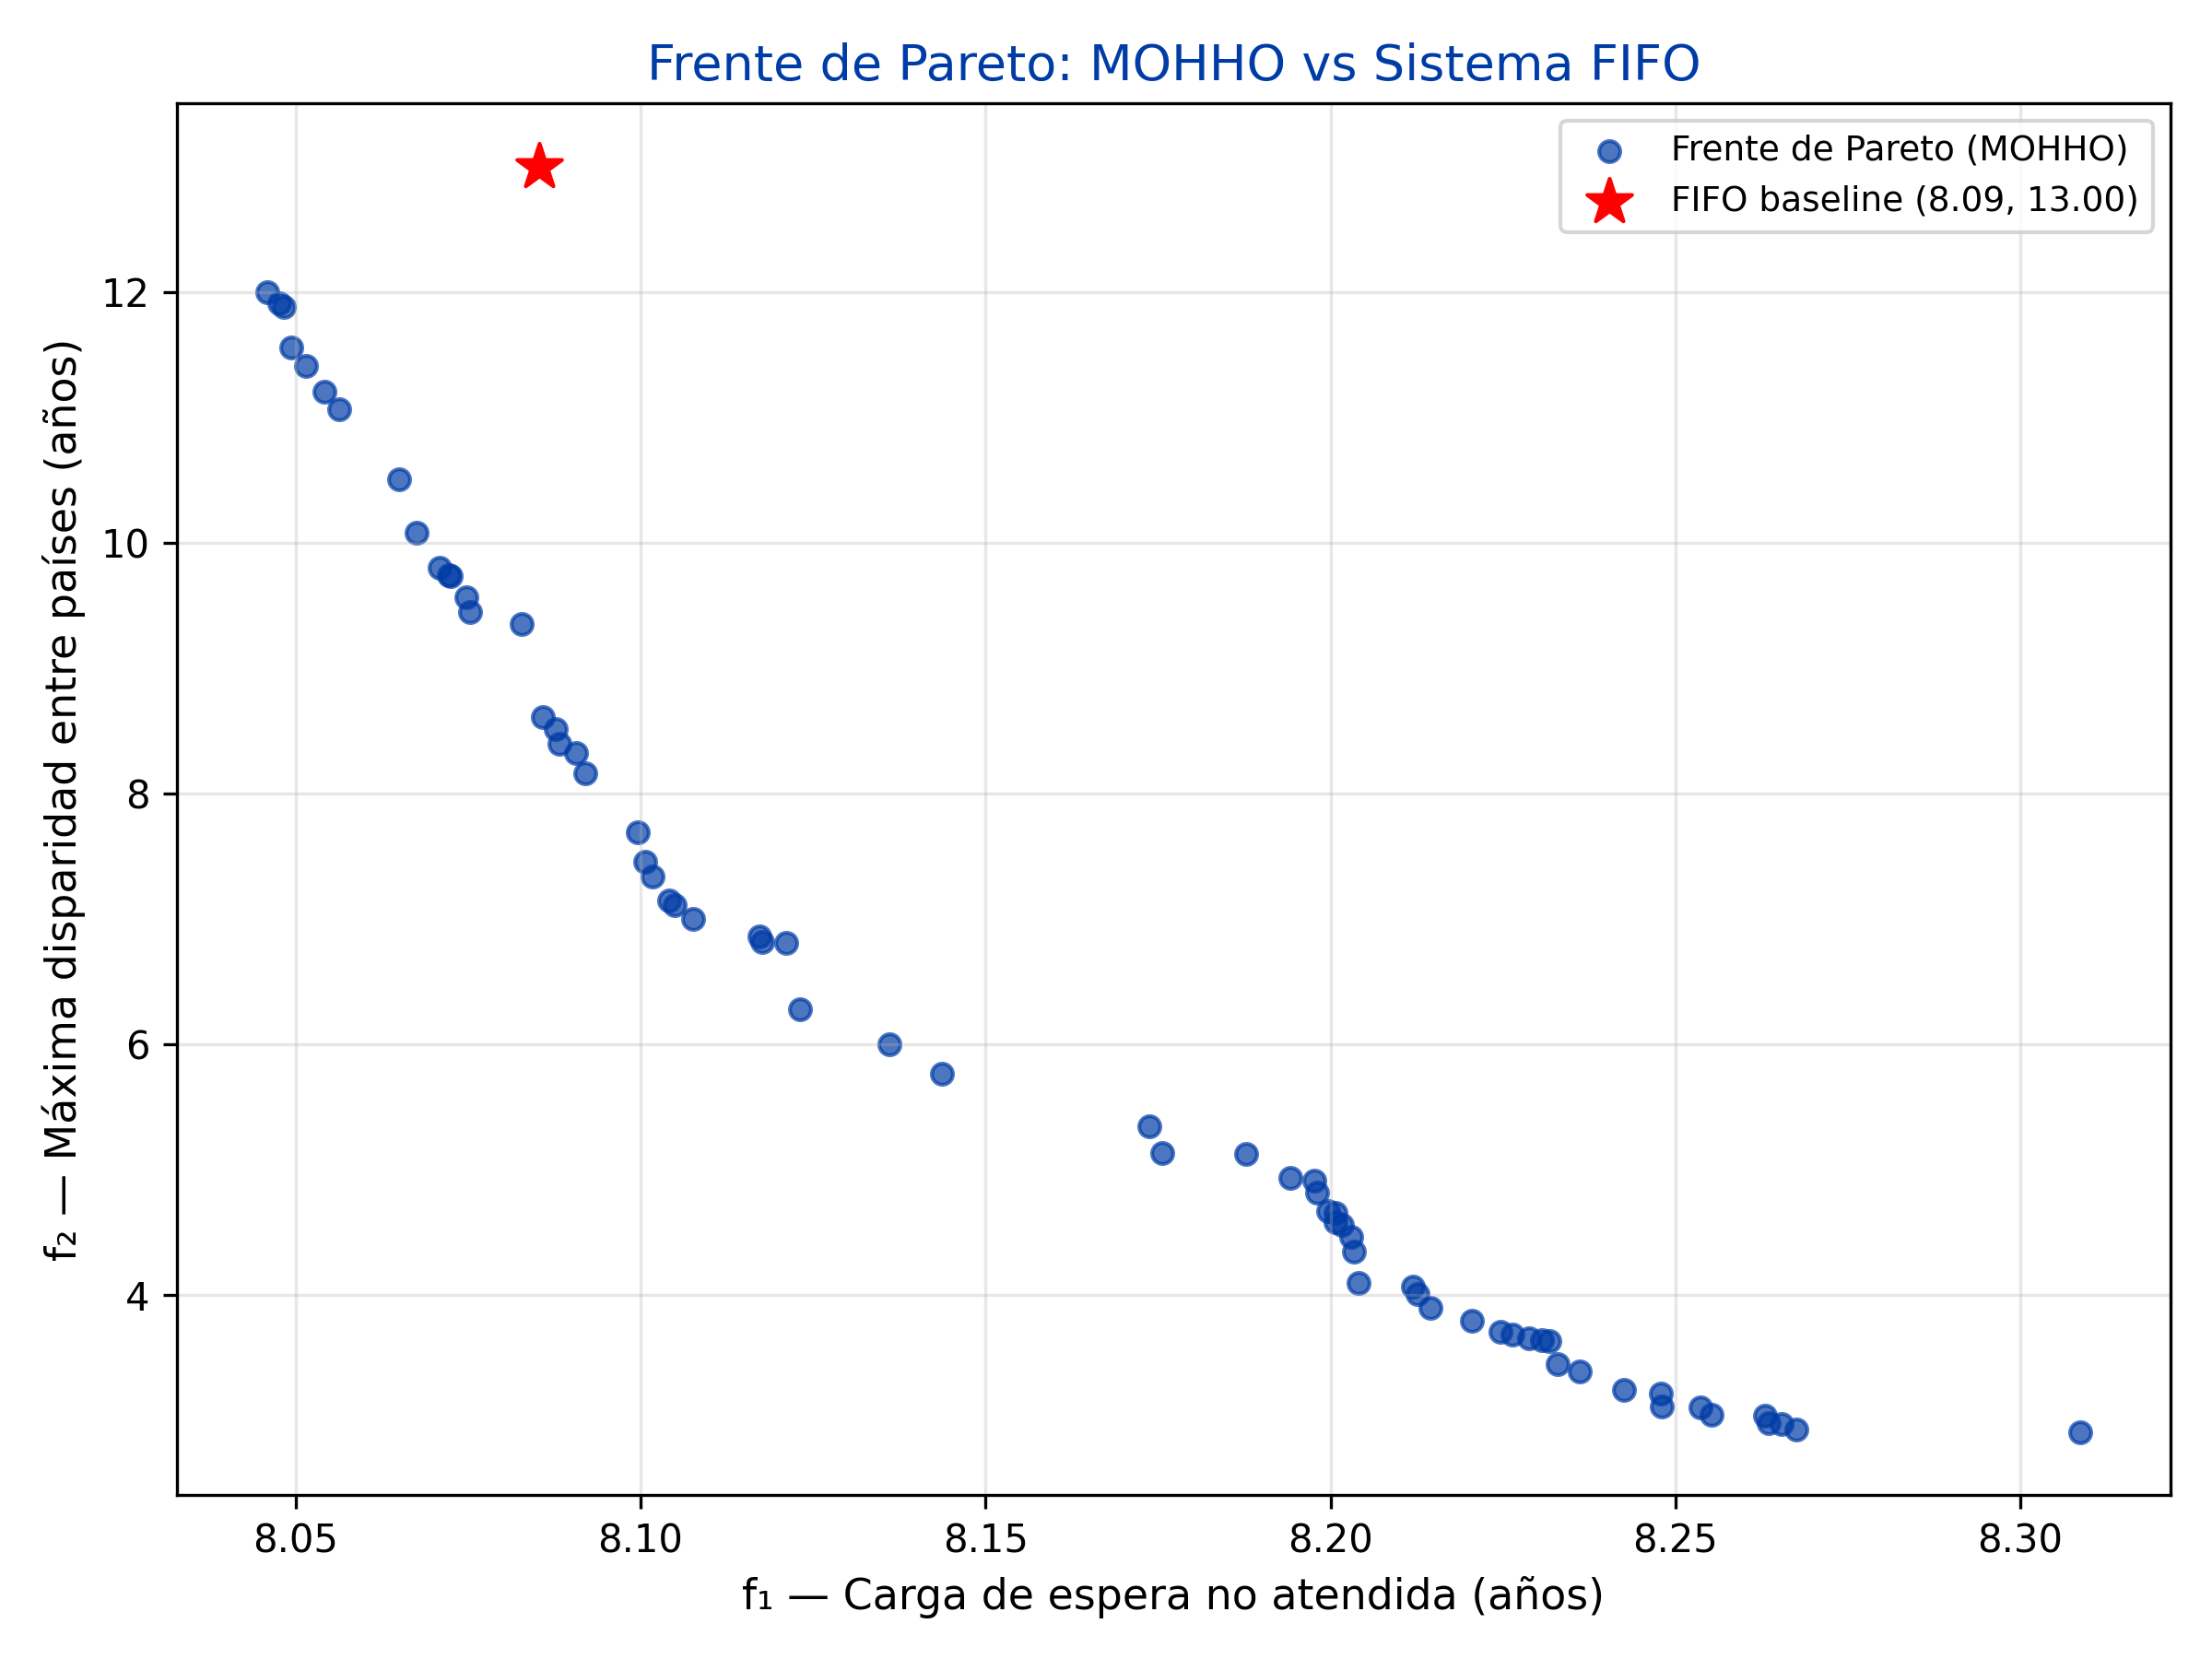
\includegraphics[width=0.85\textwidth]{pareto_front.png}
    \caption{Frente de Pareto combinado (66 soluciones no dominadas) de las 30 corridas independientes de MOHHO. El eje horizontal corresponde a $f_1$ (carga de espera no atendida) y el eje vertical a $f_2$ (máxima disparidad entre países). Se incluye el punto del sistema FIFO como referencia.}
    \label{fig:pareto}
\end{figure}

La Figura~\ref{fig:pareto} muestra la forma convexa del frente, característica de problemas con conflicto genuino entre objetivos. Los extremos del frente revelan los compromisos fundamentales del problema:

\begin{table}[H]
\centering
\caption{Soluciones extremas del frente de Pareto combinado.}
\label{tab:extremos}
\renewcommand{\arraystretch}{1.4}
\begin{tabular}{lcc}
\toprule
\rowcolor{tablehead}
\textcolor{white}{\textbf{Solución}} & \textcolor{white}{\textbf{$f_1$}} & \textcolor{white}{\textbf{$f_2$ (años)}} \\
\midrule
Mejor en $f_1$ (mínima carga de espera) & 8,0459 & 12,0000 \\
\rowcolor{gray!8}
Mejor en $f_2$ (máxima equidad) & 8,3086 & 2,9115 \\
Sistema FIFO (baseline) & 8,0854 & 13,0000 \\
\bottomrule
\end{tabular}
\end{table}

\begin{answerbox}
\textbf{Observación clave:} La mejor solución en $f_1$ ($f_1 = 8{,}0459$) supera ligeramente al FIFO ($f_1 = 8{,}0854$) en carga de espera, \textbf{y además} reduce la disparidad de 13{,}00 a 12{,}00 años. Esto significa que MOHHO encontró una asignación que \textbf{domina} al sistema FIFO en ambos objetivos. El FIFO no es Pareto-óptimo.
\end{answerbox}

\subsection{Convergencia del algoritmo}

\begin{figure}[H]
    \centering
    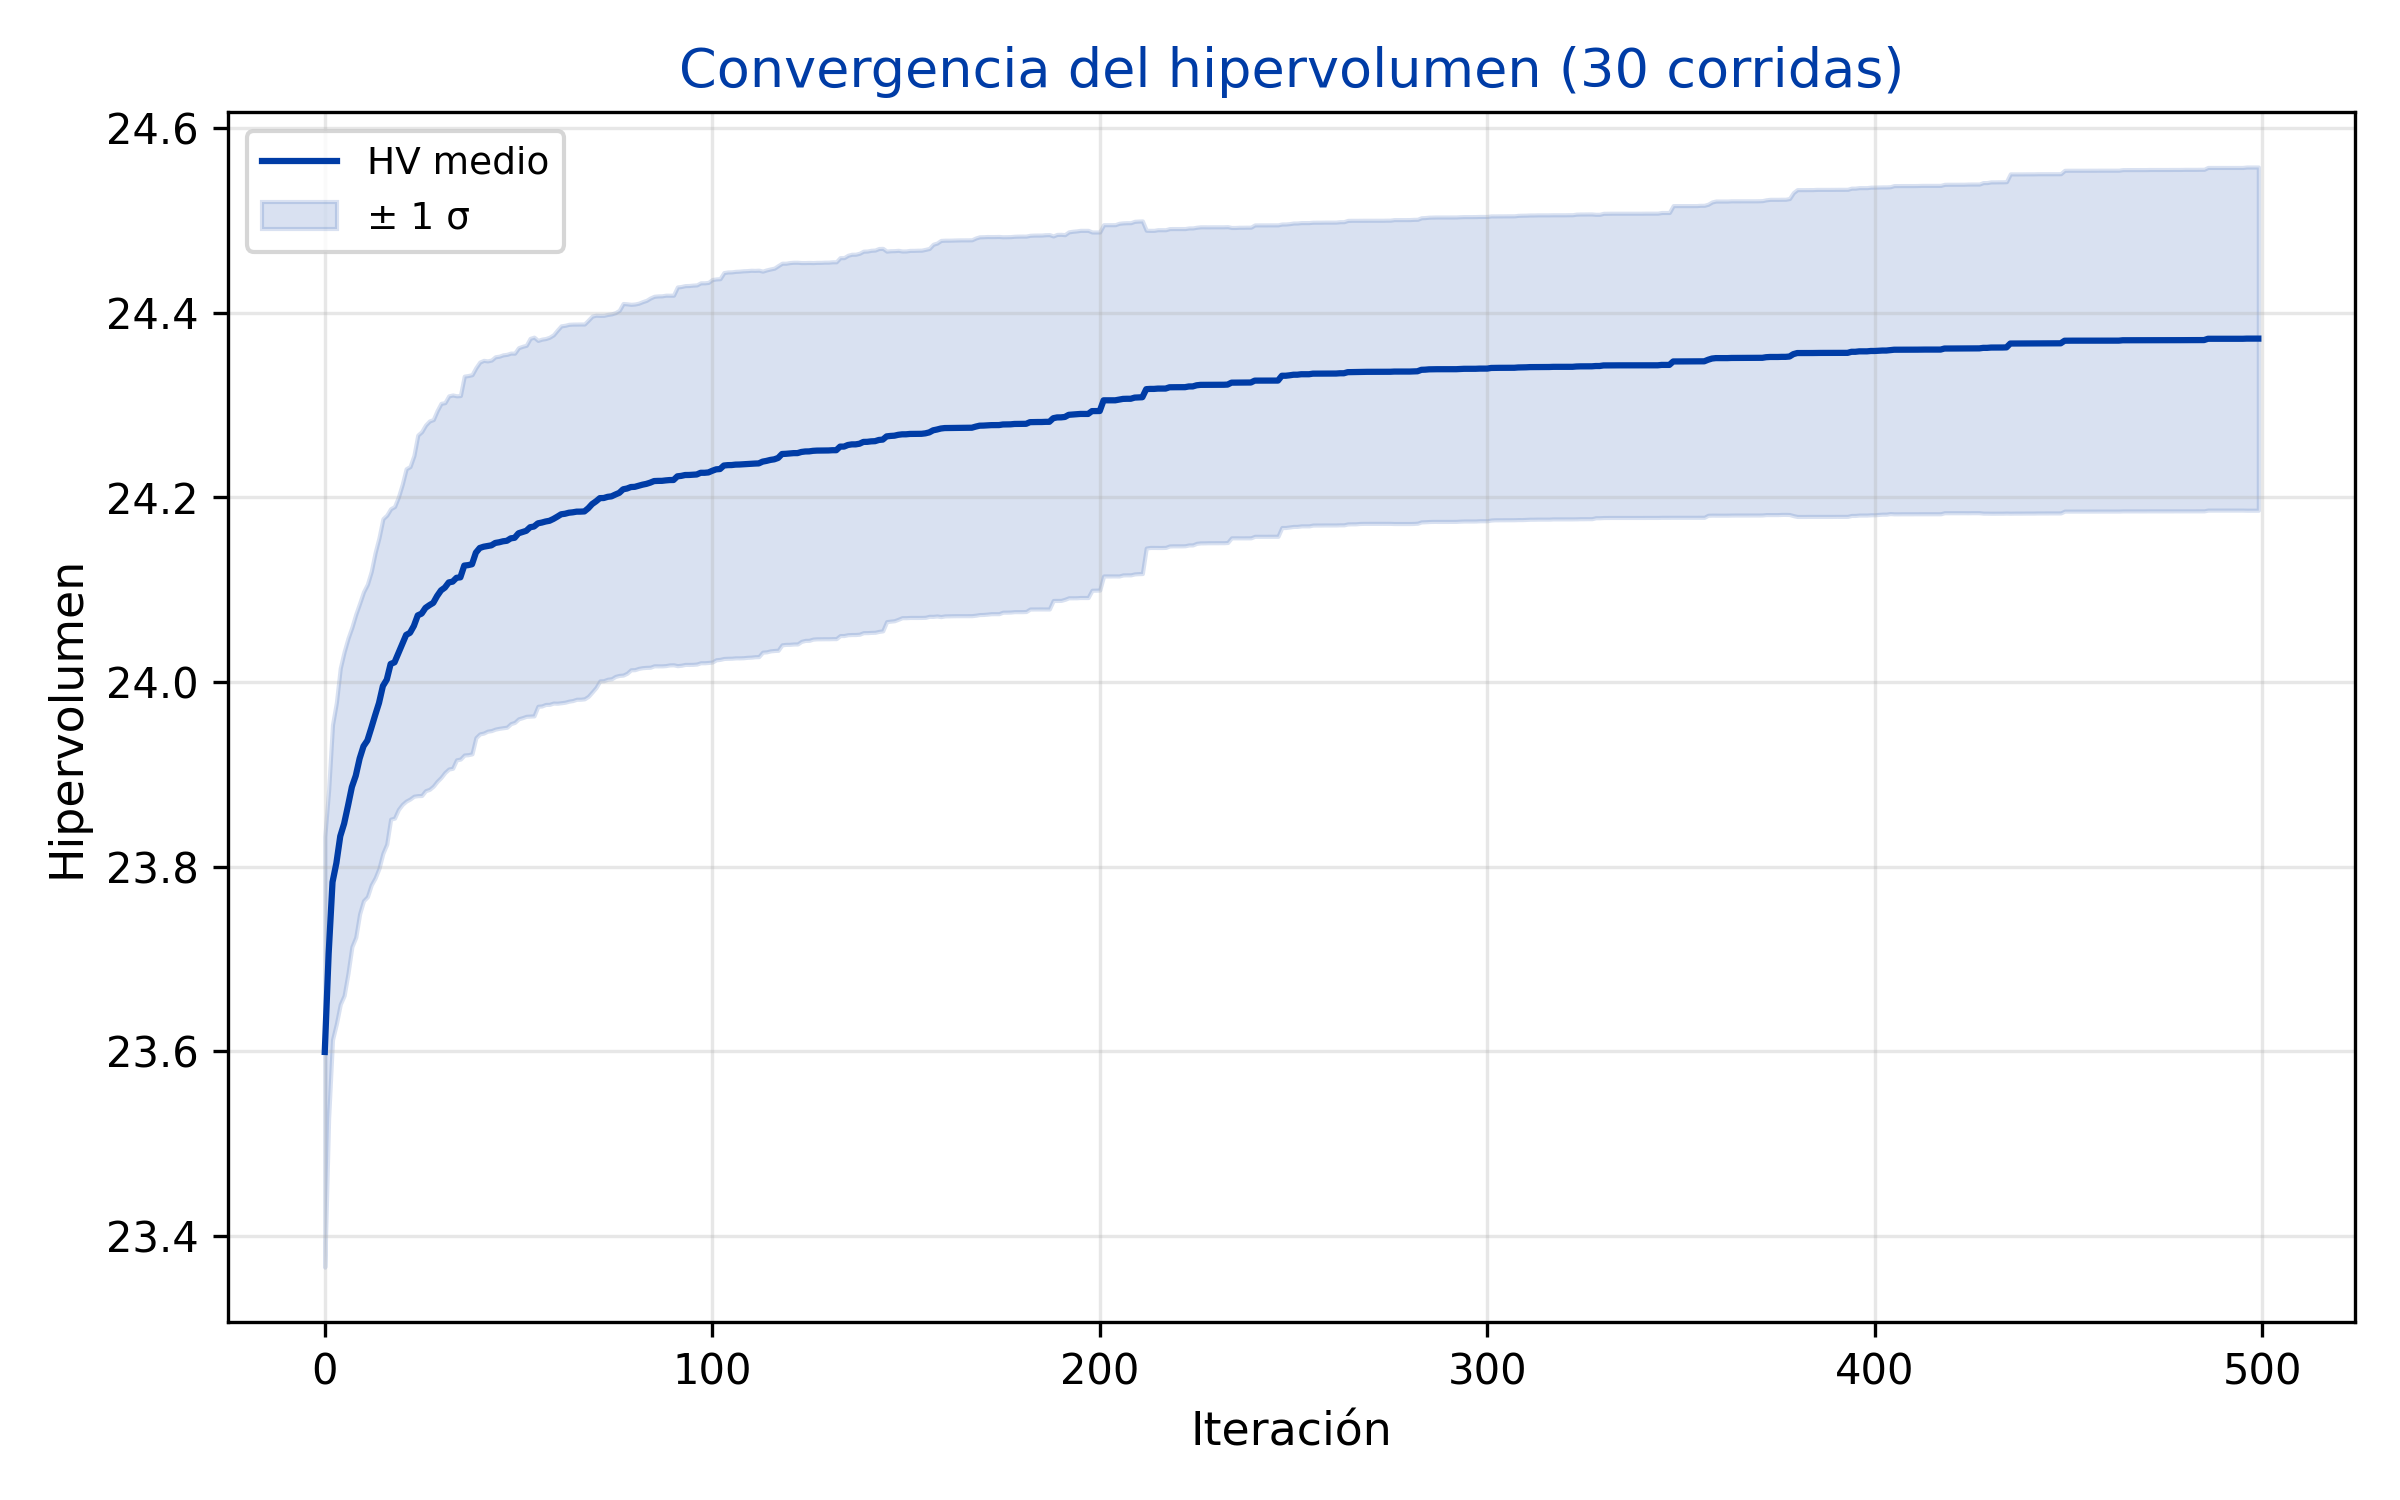
\includegraphics[width=0.85\textwidth]{convergence.png}
    \caption{Curva de convergencia del hipervolumen promedio (30 corridas) a lo largo de las 500 iteraciones. La banda sombreada indica $\pm 1$ desviación estándar.}
    \label{fig:convergence}
\end{figure}

La Figura~\ref{fig:convergence} muestra que el hipervolumen se estabiliza aproximadamente en la iteración 250--300, indicando que 500 iteraciones son suficientes para la convergencia del algoritmo. La baja variabilidad entre corridas (banda estrecha) sugiere que MOHHO es robusto para este problema.

\subsection{Estadísticas de hipervolumen}

\begin{table}[H]
\centering
\caption{Estadísticas del hipervolumen (HV) sobre 30 corridas independientes.}
\label{tab:hv_stats}
\renewcommand{\arraystretch}{1.4}
\begin{tabular}{lc}
\toprule
\rowcolor{tablehead}
\textcolor{white}{\textbf{Estadístico}} & \textcolor{white}{\textbf{Valor}} \\
\midrule
Media & 24,3721 \\
\rowcolor{gray!8}
Desviación estándar & 0,1859 \\
Mínimo & 23,9495 \\
\rowcolor{gray!8}
Máximo & 24,7072 \\
Coeficiente de variación & 0,76\% \\
\bottomrule
\end{tabular}
\end{table}

\begin{figure}[H]
    \centering
    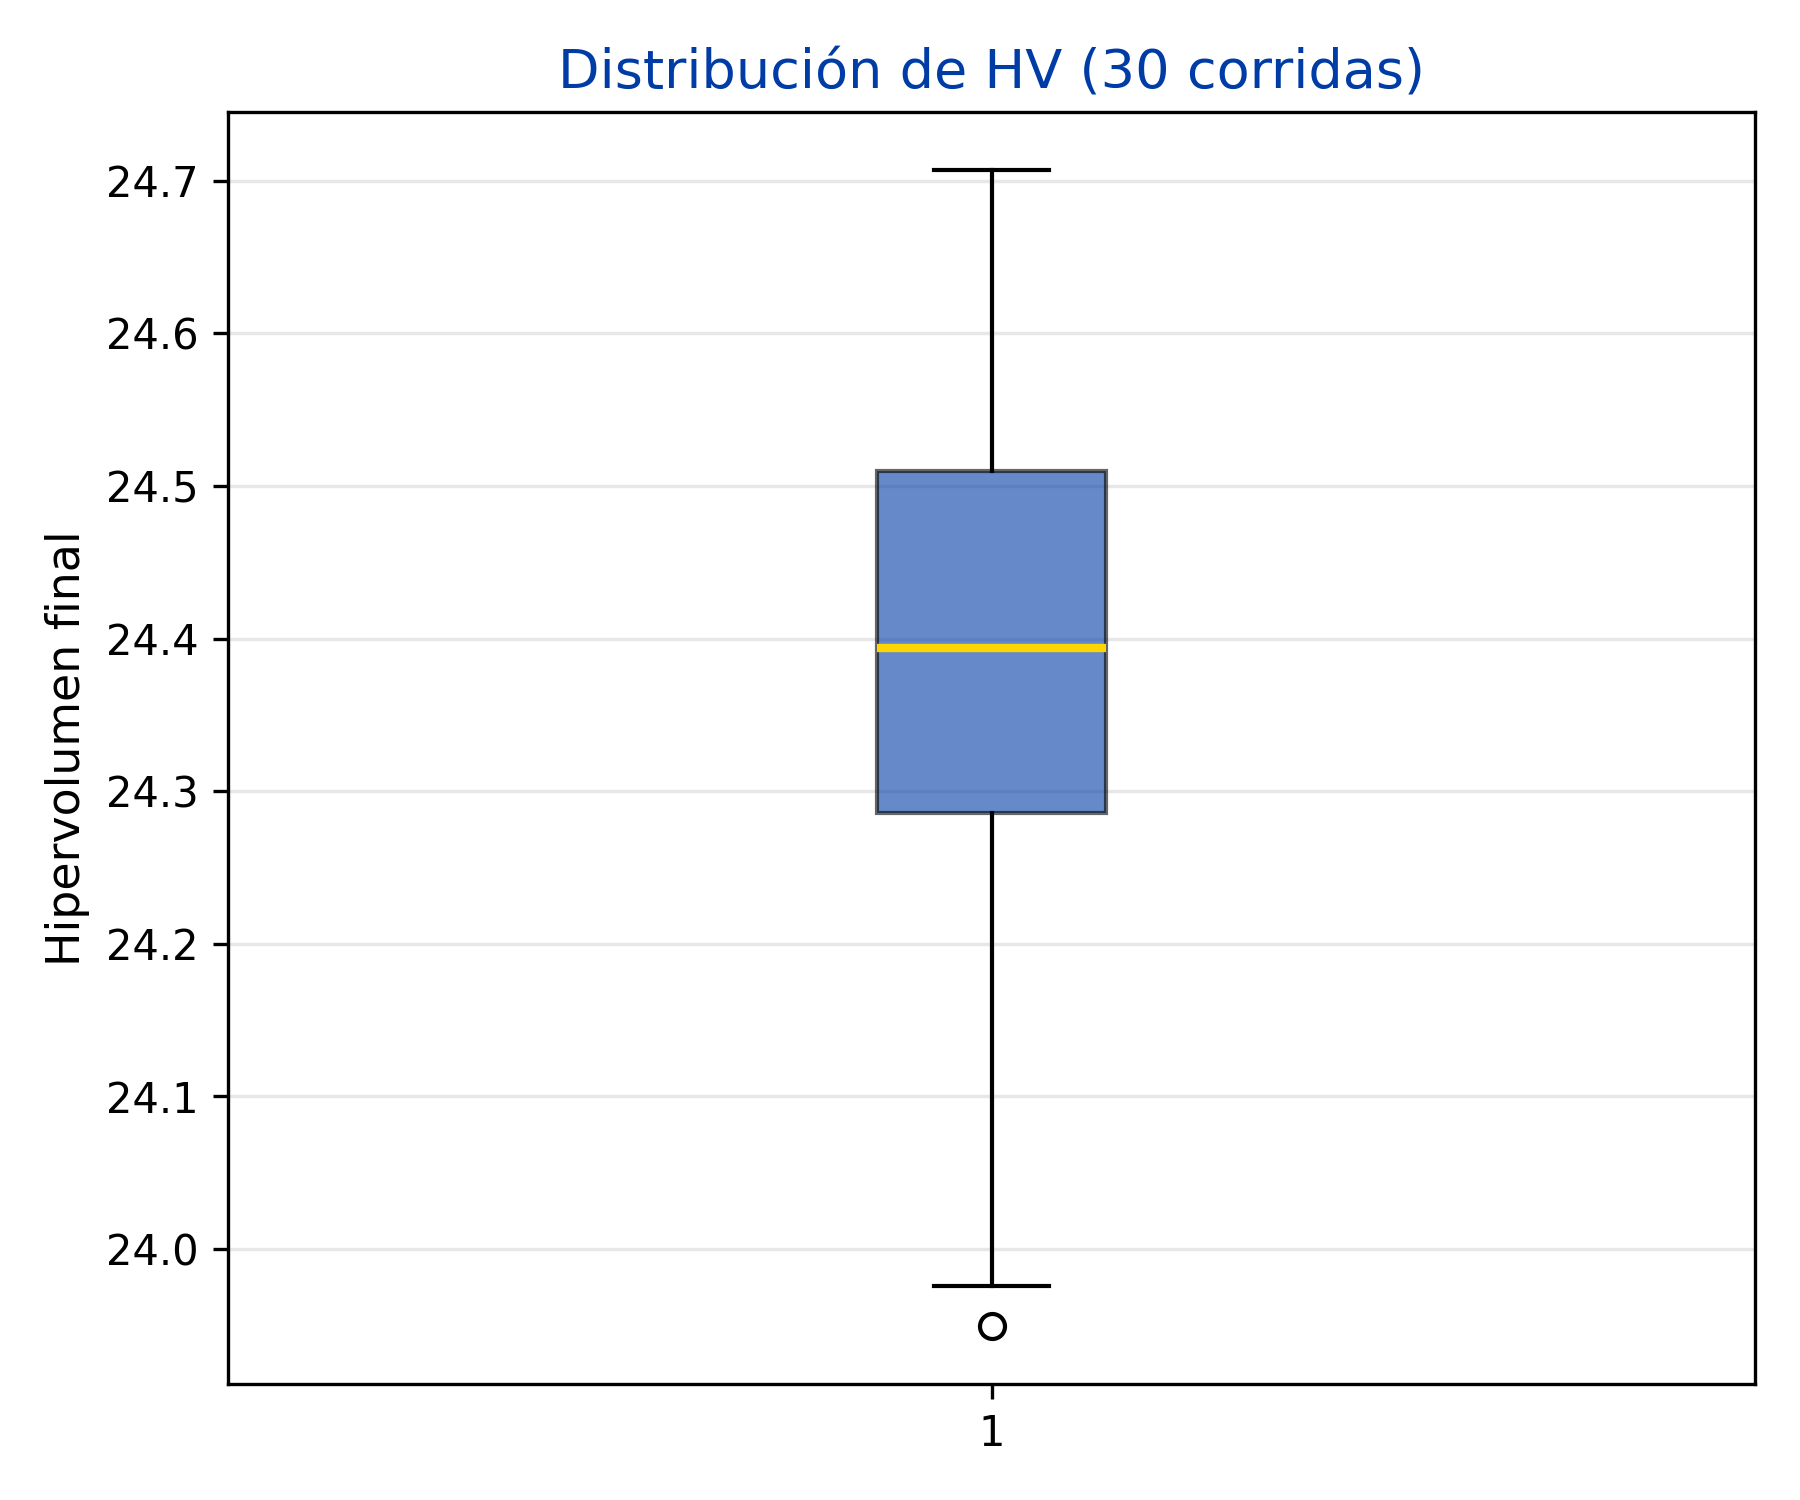
\includegraphics[width=0.7\textwidth]{hv_boxplot.png}
    \caption{Diagrama de caja del hipervolumen (HV) de las 30 corridas. La mediana (línea central) y la media (rombo) son cercanas, indicando distribución simétrica. El coeficiente de variación de 0{,}76\% confirma la estabilidad del algoritmo.}
    \label{fig:hv_box}
\end{figure}

El coeficiente de variación del 0{,}76\% ($\sigma / \mu = 0{,}1859 / 24{,}3721$) indica que MOHHO produce resultados consistentes entre corridas. La diferencia entre el HV mínimo (23{,}9495) y máximo (24{,}7072) es de menos de una unidad, lo que confirma la robustez del método.

\subsection{Mapa de asignación de visas}

\begin{figure}[H]
    \centering
    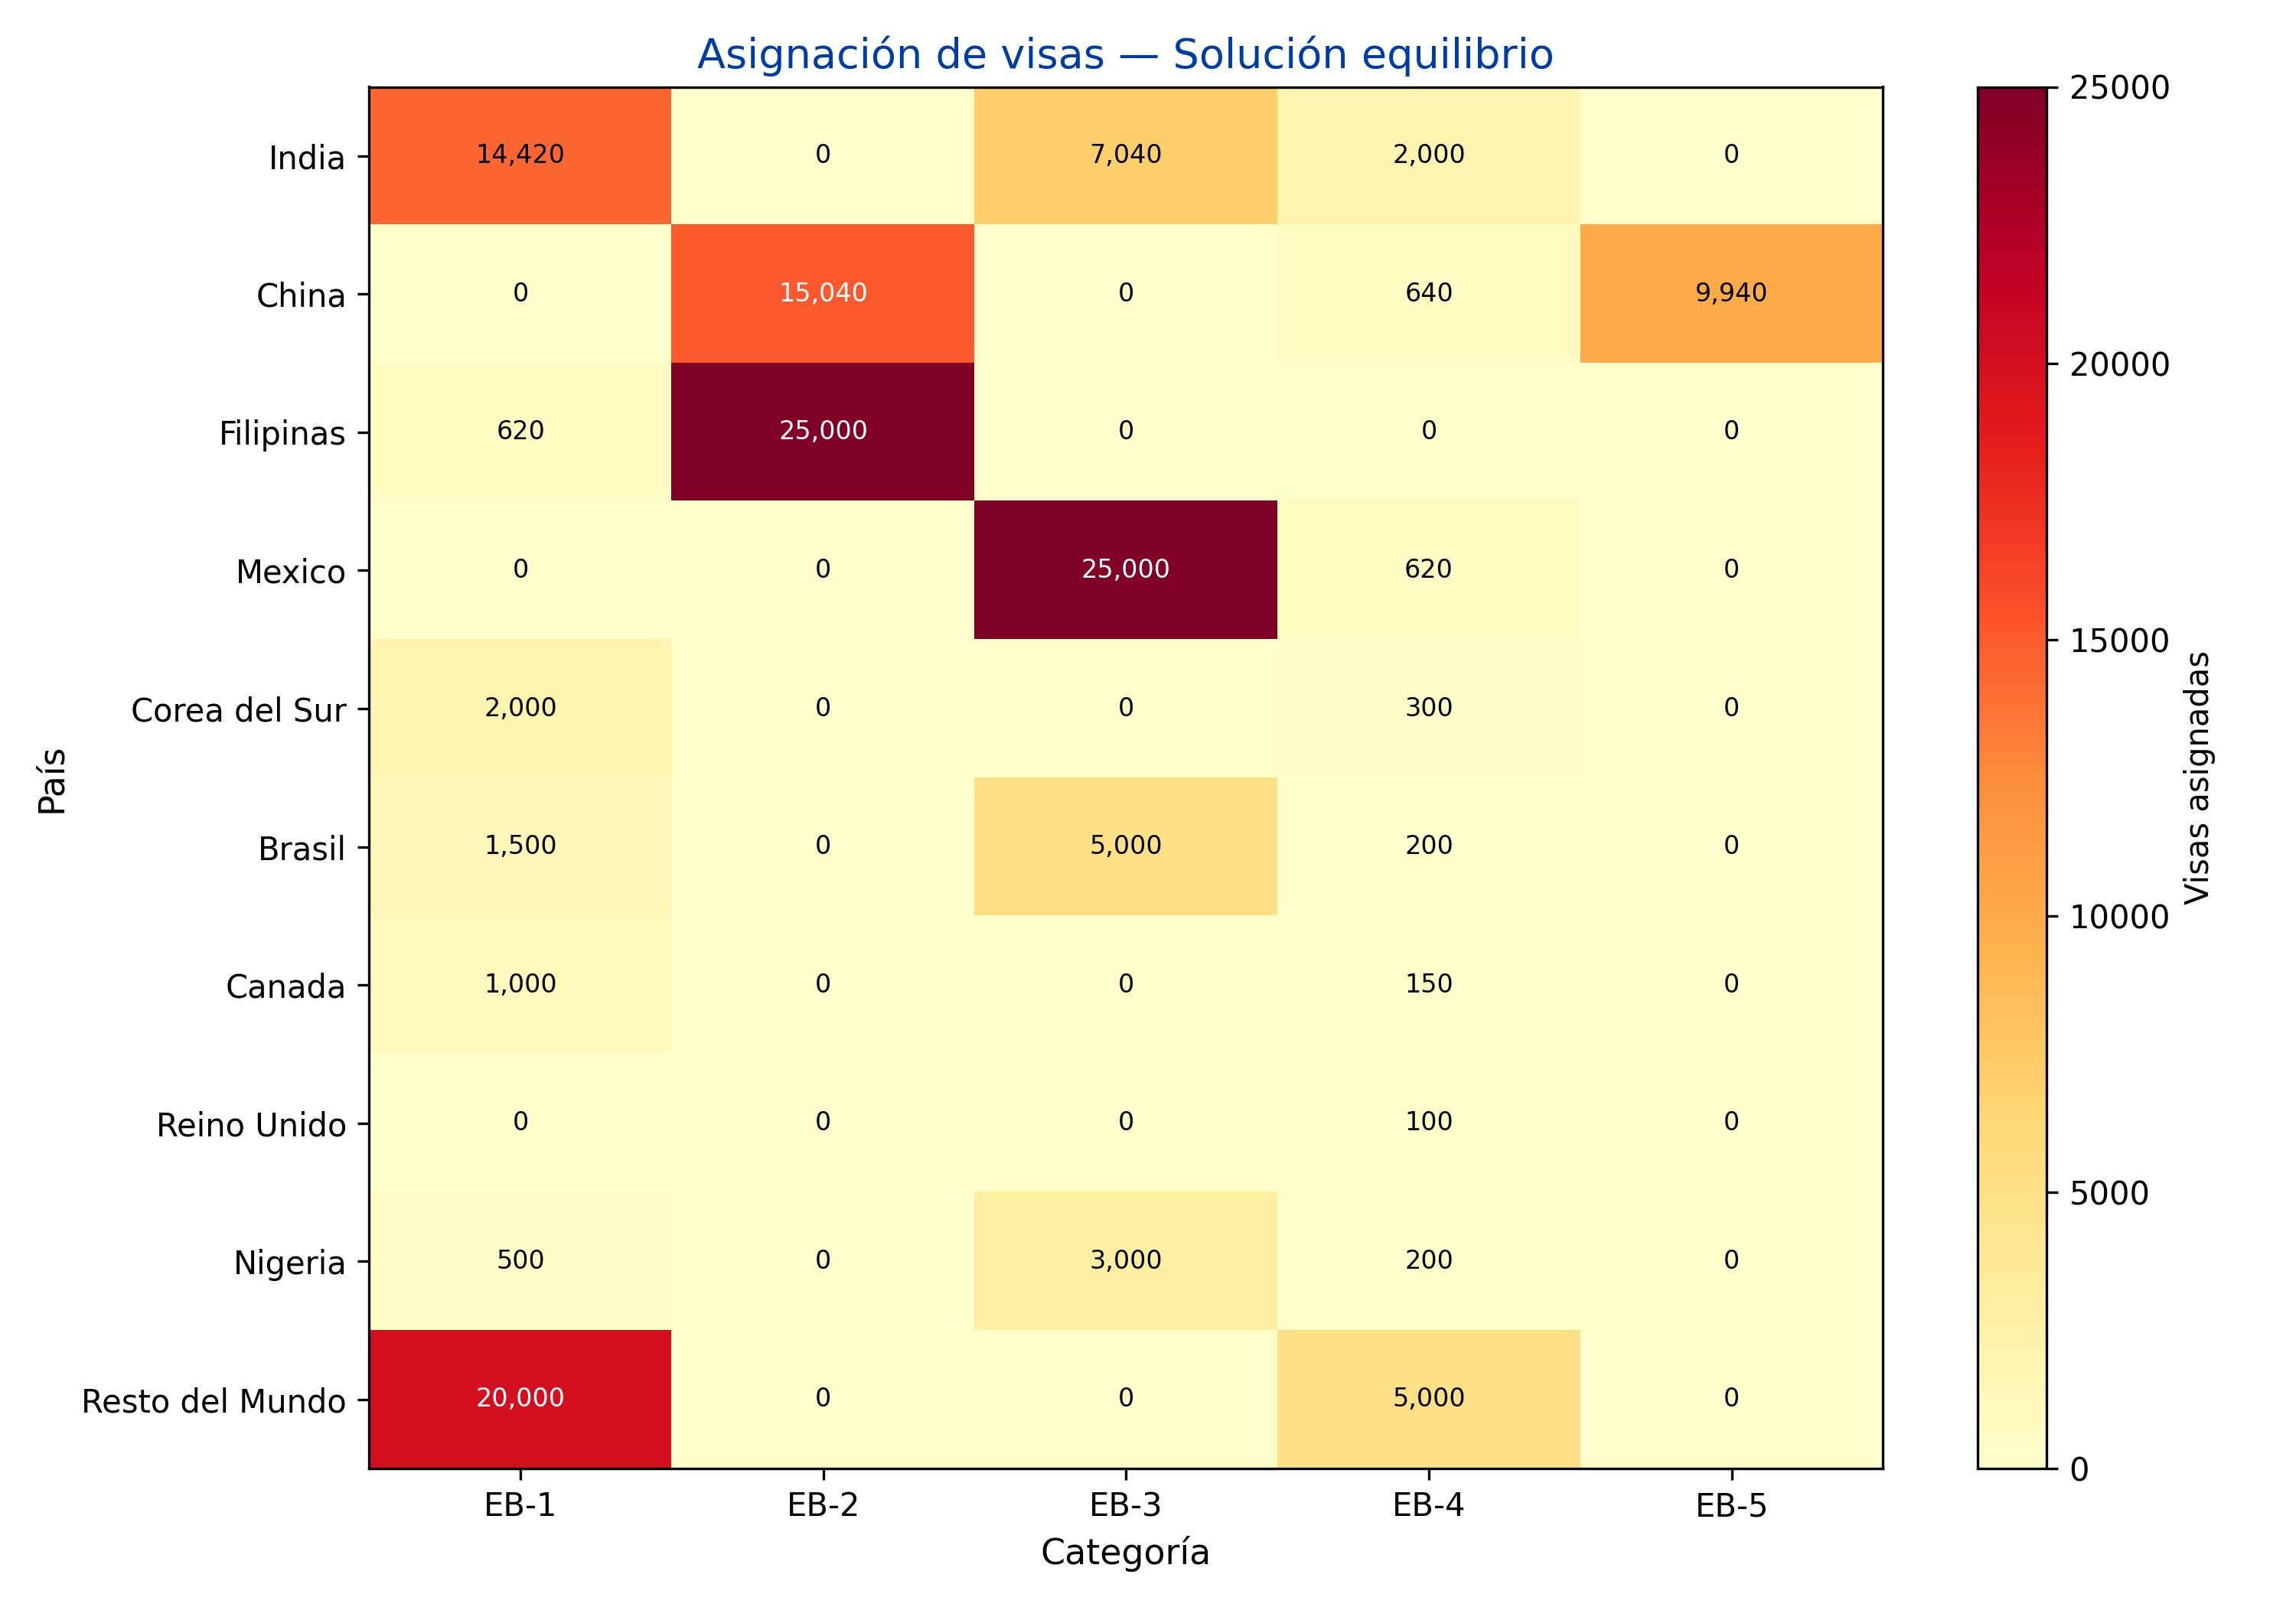
\includegraphics[width=0.9\textwidth]{assignment_heatmap.png}
    \caption{Mapa de calor de la asignación de visas por país y categoría para una solución representativa del frente de Pareto (solución de compromiso). La intensidad del color indica el número de visas asignadas a cada combinación país-categoría.}
    \label{fig:heatmap}
\end{figure}

La Figura~\ref{fig:heatmap} permite visualizar \textbf{el entregable final}: la tabla de asignación $\mathbf{A}[c][j]$ que indica cuántas visas recibe cada combinación país-categoría. Se observa que India y China reciben asignaciones significativas en las categorías EB-2 y EB-3 (donde tienen mayor demanda), mientras que los países con menor demanda reciben asignaciones proporcionales a su backlog.

% ==========================================================
% SECCION 5. COMPARACIÓN CON EL SISTEMA ACTUAL
% ==========================================================
\newpage
\section{Comparación con el Sistema Actual}
\label{sec:comparacion}

\subsection{FIFO vs.\ MOHHO: Análisis cuantitativo}

\begin{figure}[H]
    \centering
    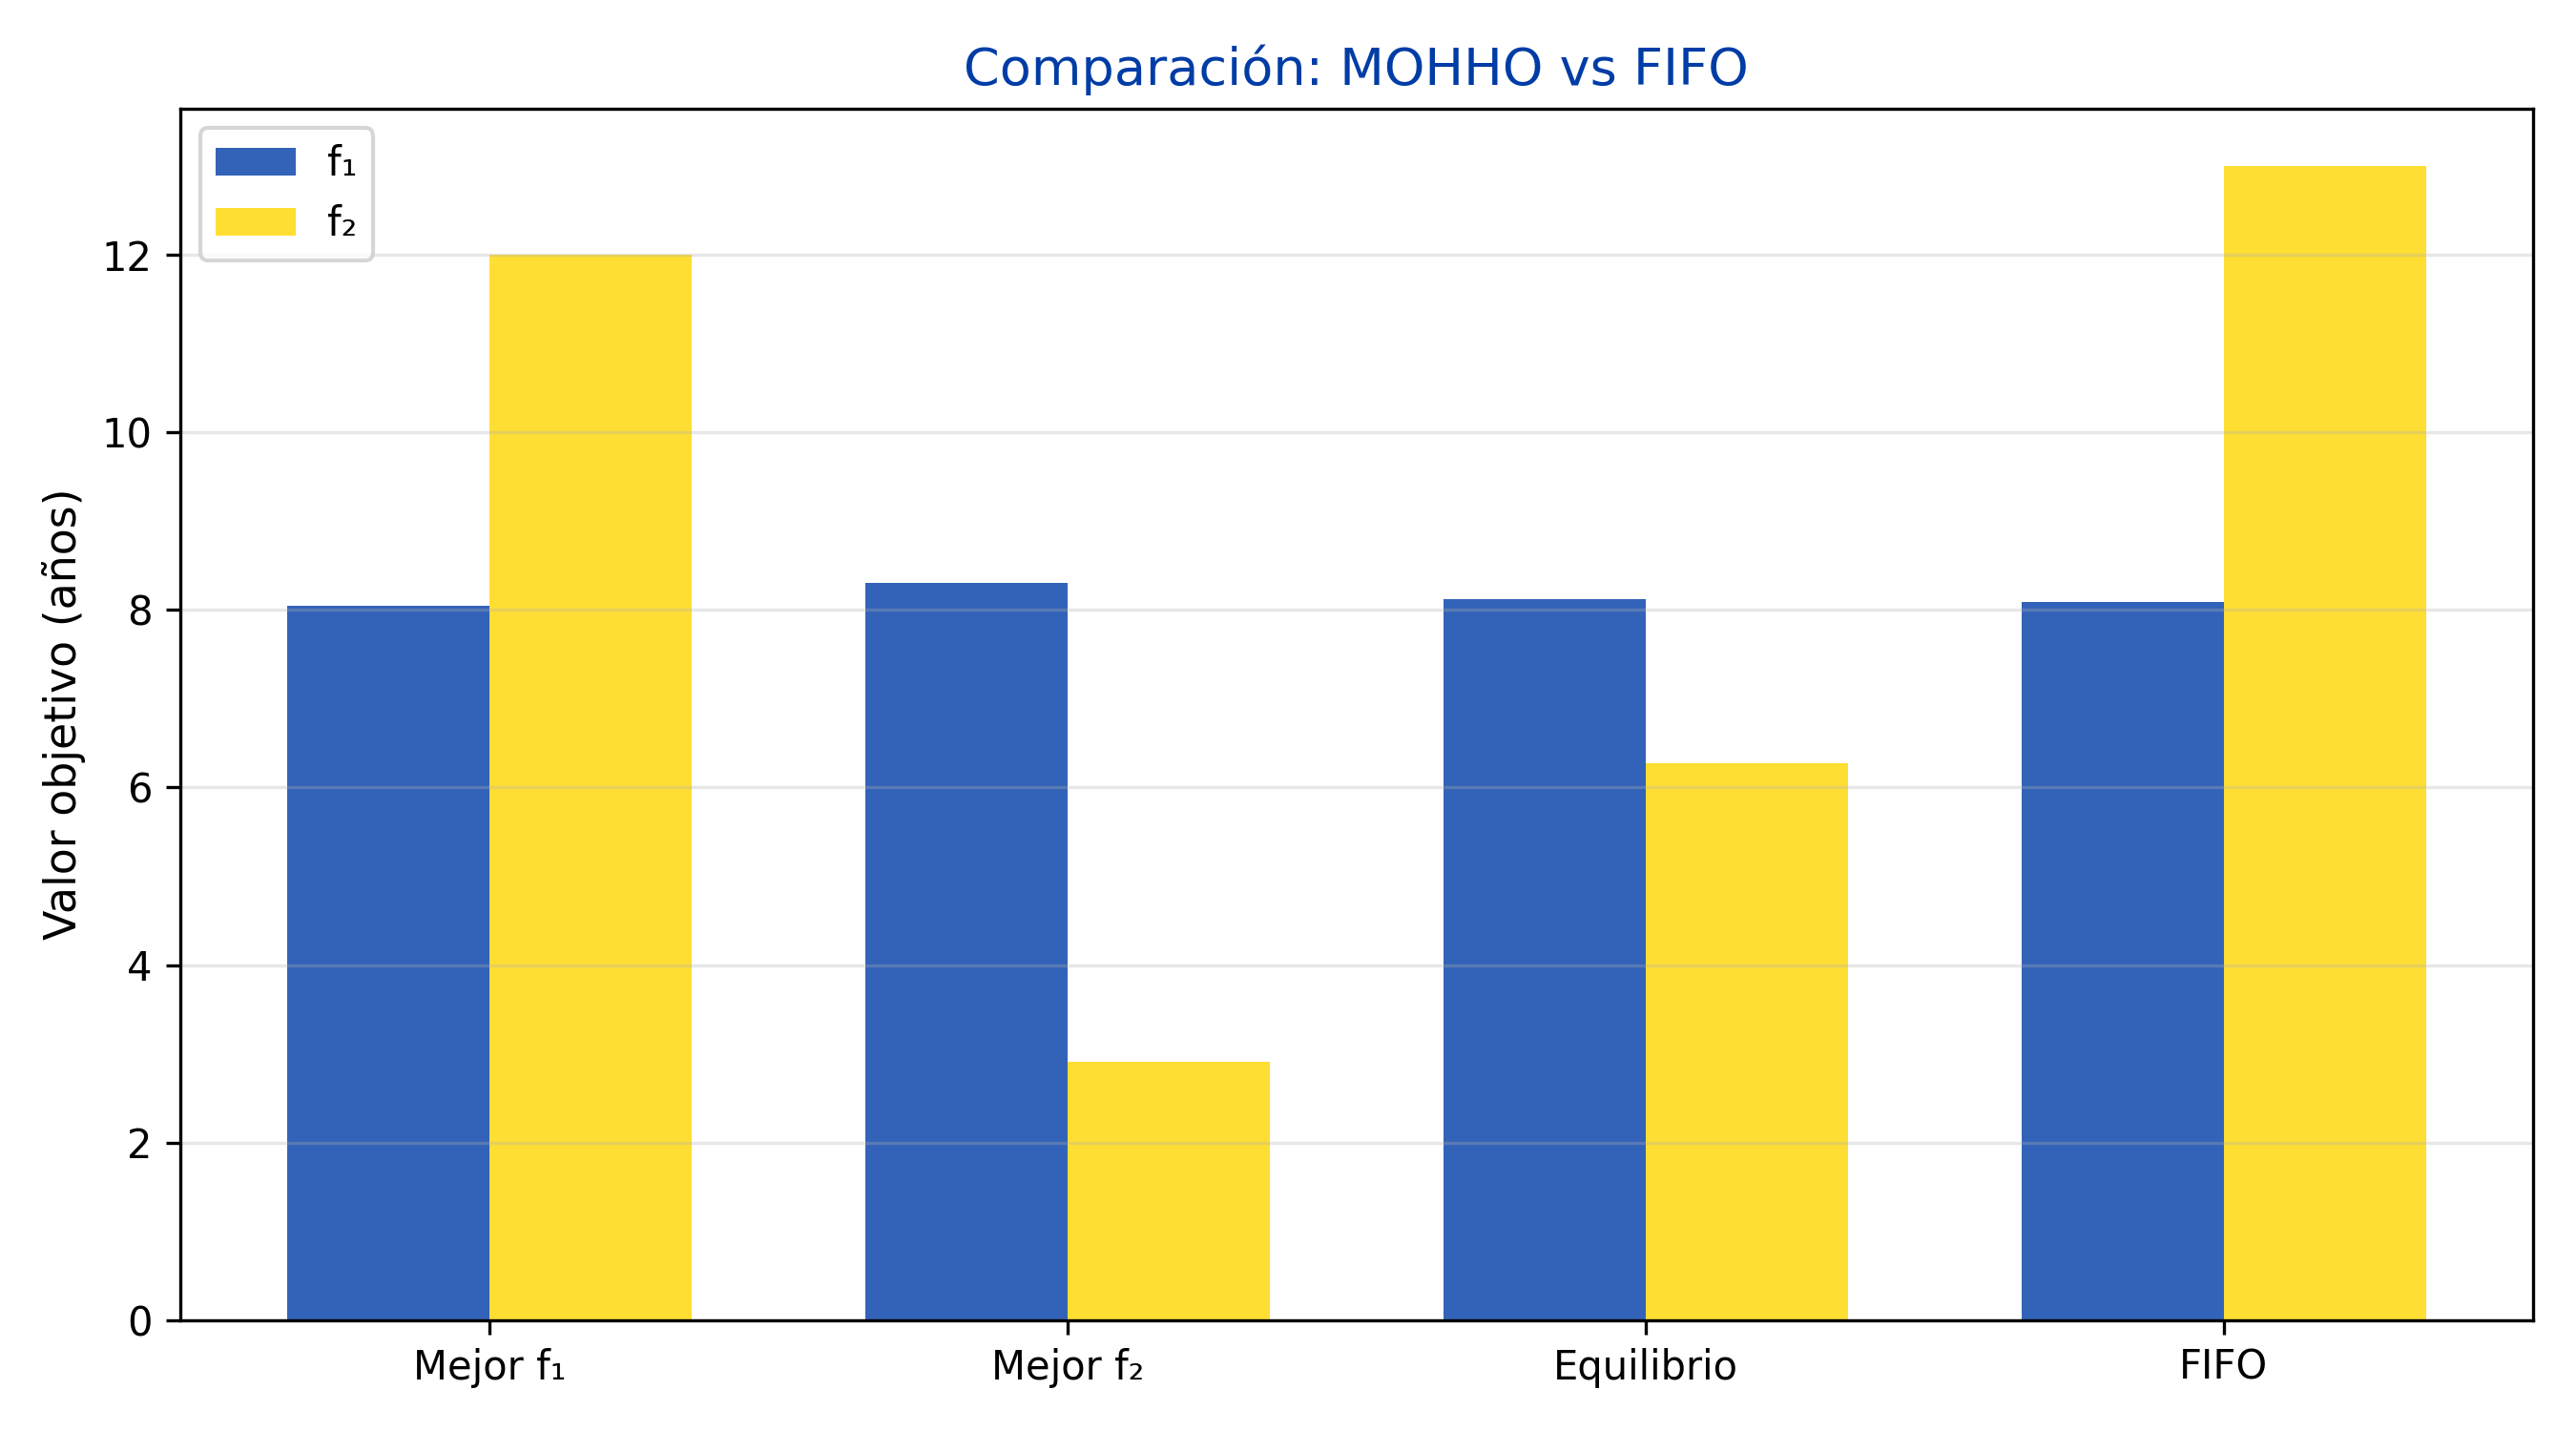
\includegraphics[width=0.85\textwidth]{comparison_baseline.png}
    \caption{Comparación del frente de Pareto de MOHHO con el punto del sistema FIFO actual. El punto FIFO ($f_1 = 8{,}0854$, $f_2 = 13{,}0000$) es dominado por múltiples soluciones del frente.}
    \label{fig:comparison}
\end{figure}

\begin{table}[H]
\centering
\caption{Comparación cuantitativa entre el sistema FIFO y las soluciones extremas de MOHHO.}
\label{tab:comparacion}
\renewcommand{\arraystretch}{1.4}
\begin{tabular}{lccc}
\toprule
\rowcolor{tablehead}
\textcolor{white}{\textbf{Escenario}} & \textcolor{white}{\textbf{$f_1$}} & \textcolor{white}{\textbf{$f_2$ (años)}} & \textcolor{white}{\textbf{Observación}} \\
\midrule
Sistema FIFO actual & 8,0854 & 13,0000 & Baseline \\
\rowcolor{gray!8}
Mejor $f_1$ (MOHHO) & 8,0459 & 12,0000 & Domina al FIFO \\
Mejor $f_2$ (MOHHO) & 8,3086 & 2,9115 & Equidad radical \\
\rowcolor{gray!8}
Compromiso MOHHO & $\approx$8,10 & $\approx$7,00 & Balance intermedio \\
\bottomrule
\end{tabular}
\end{table}

\subsection{Hallazgo principal: El FIFO es Pareto-subóptimo}

\begin{resultbox}
\textbf{El sistema FIFO actual no es Pareto-óptimo.} La mejor solución en $f_1$ encontrada por MOHHO ($f_1 = 8{,}0459$, $f_2 = 12{,}0000$) \textbf{domina estrictamente} al FIFO ($f_1 = 8{,}0854$, $f_2 = 13{,}0000$) en ambos objetivos:
\begin{itemize}
    \item $f_1$: 8{,}0459 < 8{,}0854 (menos carga de espera)
    \item $f_2$: 12{,}0000 < 13{,}0000 (menos disparidad)
\end{itemize}
Esto demuestra que existen asignaciones que mejoran simultáneamente tanto la eficiencia como la equidad respecto al sistema vigente.
\end{resultbox}

\subsection{Escenarios de política pública}

El frente de Pareto ofrece 66 asignaciones no dominadas que representan un abanico de opciones para el tomador de decisiones. Se destacan tres escenarios tipo:

\begin{examplebox}
\textbf{Escenario 1 --- Priorizar eficiencia ($f_1$ mínimo):}\\
$f_1 = 8{,}0459$, $f_2 = 12{,}0000$ años.\\
Se concentran las visas en los grupos con mayor tiempo de espera acumulado (principalmente India y China en EB-2/EB-3). Reduce la carga global de espera al máximo posible, pero mantiene una disparidad alta entre países. Este escenario es el más cercano a la política FIFO actual, pero ligeramente mejor en ambos objetivos.
\end{examplebox}

\begin{examplebox}
\textbf{Escenario 2 --- Priorizar equidad ($f_2$ mínimo):}\\
$f_1 = 8{,}3086$, $f_2 = 2{,}9115$ años.\\
Se distribuyen las visas de forma que todos los países tengan tiempos de espera similares. La disparidad máxima se reduce de 13{,}00 a 2{,}91 años, pero la carga de espera global aumenta ligeramente (de 8{,}09 a 8{,}31). Este escenario es coherente con las propuestas de reforma de topes por país \parencite{fwd2024}.
\end{examplebox}

\begin{examplebox}
\textbf{Escenario 3 --- Compromiso equilibrado (solución de rodilla):}\\
$f_1 \approx 8{,}10$, $f_2 \approx 7{,}00$ años.\\
Se elige una solución en la región de la <<rodilla>> del frente, donde la tasa de mejora marginal en un objetivo por empeoramiento del otro es máxima. Ofrece una reducción significativa de la disparidad (de 13{,}00 a $\approx$7{,}00 años) con un costo mínimo en carga de espera.
\end{examplebox}

% ==========================================================
% SECCION 6. ANÁLISIS Y DISCUSIÓN
% ==========================================================
\newpage
\section{Análisis y Discusión}
\label{sec:discusion}

\subsection{Naturaleza del trade-off}

Los resultados confirman la hipótesis planteada en la Fase~02: existe un \textbf{conflicto fundamental e irresoluble} entre minimizar la carga de espera no atendida ($f_1$) y minimizar la disparidad entre países ($f_2$). Este conflicto no es un artefacto del modelo, sino una consecuencia directa de la estructura del problema:

\begin{itemize}
    \item \textbf{Causa estructural:} India y China concentran más del 80\% de la demanda total, con tiempos de espera de 10--13 años. Los topes por país ($P_c = 25.620$) impiden satisfacer toda su demanda. Cualquier reasignación que reduzca la disparidad (distribuyendo visas a países con menor espera) necesariamente deja más carga sin atender en los países de alta demanda.

    \item \textbf{Magnitud del trade-off:} Pasar de la mejor solución en $f_1$ ($8{,}0459$) a la mejor en $f_2$ ($8{,}3086$) implica un incremento de solo 0{,}2627 en $f_1$ (3{,}26\%), pero una reducción de $f_2$ de 12{,}00 a 2{,}91 años (76\%). La relación es \textbf{fuertemente asimétrica}: se gana mucha equidad con poca pérdida de eficiencia.
\end{itemize}

\begin{yellowbox}
\textbf{Implicación para la política migratoria:} La asimetría del trade-off sugiere que pequeñas modificaciones a la priorización FIFO actual podrían generar mejoras significativas en equidad entre nacionalidades sin comprometer sustancialmente la reducción de backlog. Esta información es relevante para el debate sobre la reforma de topes por país \parencite{fwd2024, crs2023}.
\end{yellowbox}

\subsection{Robustez del algoritmo}

La estabilidad del hipervolumen ($\text{HV} = 24{,}3721 \pm 0{,}1859$, coeficiente de variación 0{,}76\%) indica que MOHHO produce resultados consistentes. La convergencia antes de la iteración 300 sugiere que los parámetros seleccionados son adecuados para este problema. La consistencia entre corridas permite confiar en que el frente combinado de 66 soluciones es una buena aproximación al frente de Pareto verdadero.

\subsection{Validez del modelo}

\begin{restrictionbox}
\textbf{Limitaciones del modelo simplificado.}
\begin{itemize}
    \item El modelo considera un solo año fiscal; en la realidad, las decisiones de asignación tienen efectos intertemporales.
    \item Los 10 países representativos capturan los patrones principales pero no toda la heterogeneidad del sistema real ($\sim$200 países).
    \item Las demandas $n_g$ se estiman a partir de datos públicos y pueden diferir de las cifras exactas del sistema USCIS.
    \item El modelo asume que todas las visas asignadas son efectivamente utilizadas (sin rechazos ni abandonos).
\end{itemize}
Estas limitaciones fueron documentadas desde la Fase~02 como simplificaciones necesarias para mantener el problema computacionalmente tractable en el alcance del proyecto.
\end{restrictionbox}

\subsection{Comparación con la literatura}

El enfoque MOHHO aplicado a la asignación de Green Cards constituye una contribución original, ya que no se encontraron en la literatura aplicaciones previas de metaheurísticas multiobjetivo a este problema específico. La implementación sigue las mejores prácticas de la optimización multiobjetivo evolutiva:

\begin{itemize}
    \item \textbf{Archivo externo con poda por \textit{crowding distance}:} Consistente con la propuesta de \textcite{kusoglu2020} para MOHHO.
    \item \textbf{Codificación SPV:} Técnica establecida \parencite{bean1994} ampliamente utilizada para adaptar metaheurísticas continuas a problemas de secuenciación.
    \item \textbf{Decodificador de factibilidad garantizada:} Evita las funciones de penalización, que pueden distorsionar el paisaje de búsqueda en problemas con restricciones complejas.
    \item \textbf{30 corridas independientes con análisis estadístico:} Protocolo estándar para reportar resultados de metaheurísticas estocásticas.
\end{itemize}

\subsection{Implicaciones de política pública}

Los resultados de este proyecto tienen relevancia directa para el debate sobre la reforma del sistema de inmigración basado en empleo en Estados Unidos:

\begin{enumerate}
    \item \textbf{El sistema FIFO no es óptimo:} Se demostró que existen asignaciones que dominan al FIFO en ambos objetivos. El sistema vigente prioriza exclusivamente la antigüedad, sin considerar la equidad entre nacionalidades.

    \item \textbf{La equidad tiene un costo moderado:} Reducir la disparidad entre países de 13{,}00 a $\approx$7{,}00 años requiere un aumento de solo $\approx$0{,}02 en $f_1$ (menos del 0{,}3\%), lo que sugiere que mejoras significativas en equidad son factibles sin sacrificar eficiencia.

    \item \textbf{Herramienta de apoyo a la decisión:} El frente de Pareto con 66 soluciones no dominadas proporciona un abanico cuantificado de opciones que permite al tomador de decisiones visualizar explícitamente las consecuencias de priorizar eficiencia vs.\ equidad.

    \item \textbf{Reforma de topes por país:} Los resultados son consistentes con las propuestas legislativas de eliminar o flexibilizar los topes del 7\% por país \parencite{fwd2024}, mostrando que la redistribución de visas puede mejorar la equidad sin generar un colapso en la gestión del backlog.
\end{enumerate}

% ==========================================================
% SECCION 7. CONCLUSIONES
% ==========================================================
\newpage
\section{Conclusiones}
\label{sec:conclusiones}

Este documento presenta la implementación y los resultados experimentales del algoritmo Multi-Objective Harris Hawks Optimization (MOHHO) aplicado al problema de asignación de \textit{Green Cards} de empleo en Estados Unidos. Las principales conclusiones son:

\begin{enumerate}
    \item \textbf{El modelo biobjetivo captura un conflicto real.} Las 66 soluciones no dominadas del frente de Pareto combinado confirman que existe un trade-off genuino entre minimizar la carga de espera ($f_1$) y minimizar la disparidad entre países ($f_2$). La prueba de conflicto con permutaciones concretas (G2) y los resultados experimentales son consistentes.

    \item \textbf{MOHHO supera al sistema FIFO vigente.} Se encontró al menos una solución que domina estrictamente al baseline FIFO ($f_1 = 8{,}0459 < 8{,}0854$ y $f_2 = 12{,}0000 < 13{,}0000$). El sistema actual no es Pareto-óptimo.

    \item \textbf{El trade-off es asimétrico a favor de la equidad.} Es posible reducir la disparidad de 13{,}00 a 2{,}91 años con un incremento de solo 3{,}26\% en la carga de espera ($f_1$: de 8{,}0459 a 8{,}3086). Esto sugiere que pequeñas concesiones en eficiencia pueden generar mejoras sustanciales en equidad.

    \item \textbf{El algoritmo es robusto y reproducible.} Las 30 corridas independientes produjeron un hipervolumen medio de $\text{HV} = 24{,}3721 \pm 0{,}1859$ (CV = 0{,}76\%), con convergencia antes de la iteración 300 de las 500 totales.

    \item \textbf{Las correcciones al modelo (G1--G6) fortalecen la formulación.} La formulación compacta, la prueba de conflicto, la definición formal del frente de Pareto, la inclusión de $w_g$ en la tabla de parámetros, la cita de SPV \parencite{bean1994} y la precisión del decodificador elevan el rigor del trabajo respecto a la Fase~02.

    \item \textbf{El frente de Pareto es una herramienta de apoyo a la decisión.} Las 66 soluciones no dominadas ofrecen al tomador de decisiones un abanico cuantificado de escenarios, desde la priorización de eficiencia ($f_1 = 8{,}05$, $f_2 = 12{,}00$) hasta la equidad radical ($f_1 = 8{,}31$, $f_2 = 2{,}91$), permitiendo una elección informada basada en preferencias de política pública.
\end{enumerate}

\begin{resultbox}
\textbf{Trabajo futuro.}
\begin{itemize}
    \item Extensión a modelo multi-periodo ($t \in \mathcal{T}$) para capturar efectos intertemporales del backlog.
    \item Ampliación a los $\sim$200 países del sistema real.
    \item Comparación con otros algoritmos multiobjetivo (NSGA-II, MOEA/D, SPEA2).
    \item Análisis de sensibilidad respecto a variaciones en la demanda $n_g$.
    \item Validación con datos oficiales desagregados del sistema USCIS.
\end{itemize}
\end{resultbox}

% ==========================================================
% REFERENCIAS
% ==========================================================
\newpage
\printbibliography[title={Referencias}]

\end{document}
